
% !TeX spellcheck = de_DE

\documentclass{article}

\usepackage[ngerman]{babel}
\usepackage{graphicx}
\usepackage{indentfirst}
\usepackage{hyperref}
\usepackage{geometry}
\usepackage{changepage}
\usepackage{booktabs}
\usepackage{float}
\usepackage{tabulary}
\usepackage{xcolor}
\usepackage{multirow}
\usepackage{caption}
\usepackage{subcaption}
\usepackage{lscape}
\usepackage{colortbl}
\usepackage{listings}

\graphicspath{ {./images/} }
\setlength\parindent{0pt}

\makeatletter
\newcommand{\sectionauthor}[1]{
	{\parindent 0em \large \scshape Autor: #1 \par \nobreak \vspace*{1em}}
	\@afterheading
}
\newcommand{\specification}[3]{
	{\parindent 0.5em \hangindent 3em \hypertarget{spec:#1:#2}{\textbf{/#1#2/}} #3 \par \nobreak \vspace*{0.5em}}
}
\makeatother

\title{Bibliotheksanwendung - Feinspezifikation}
\date{\today\\v1.1}
\author{
	Ivan Charviakou\\
	León Liehr\\
	Mohamad Najjar\\
	Jonas Picker\\
	Sergei Pravdin
}

\begin{document}
\maketitle
\begin{figure}[H]
	\centering
	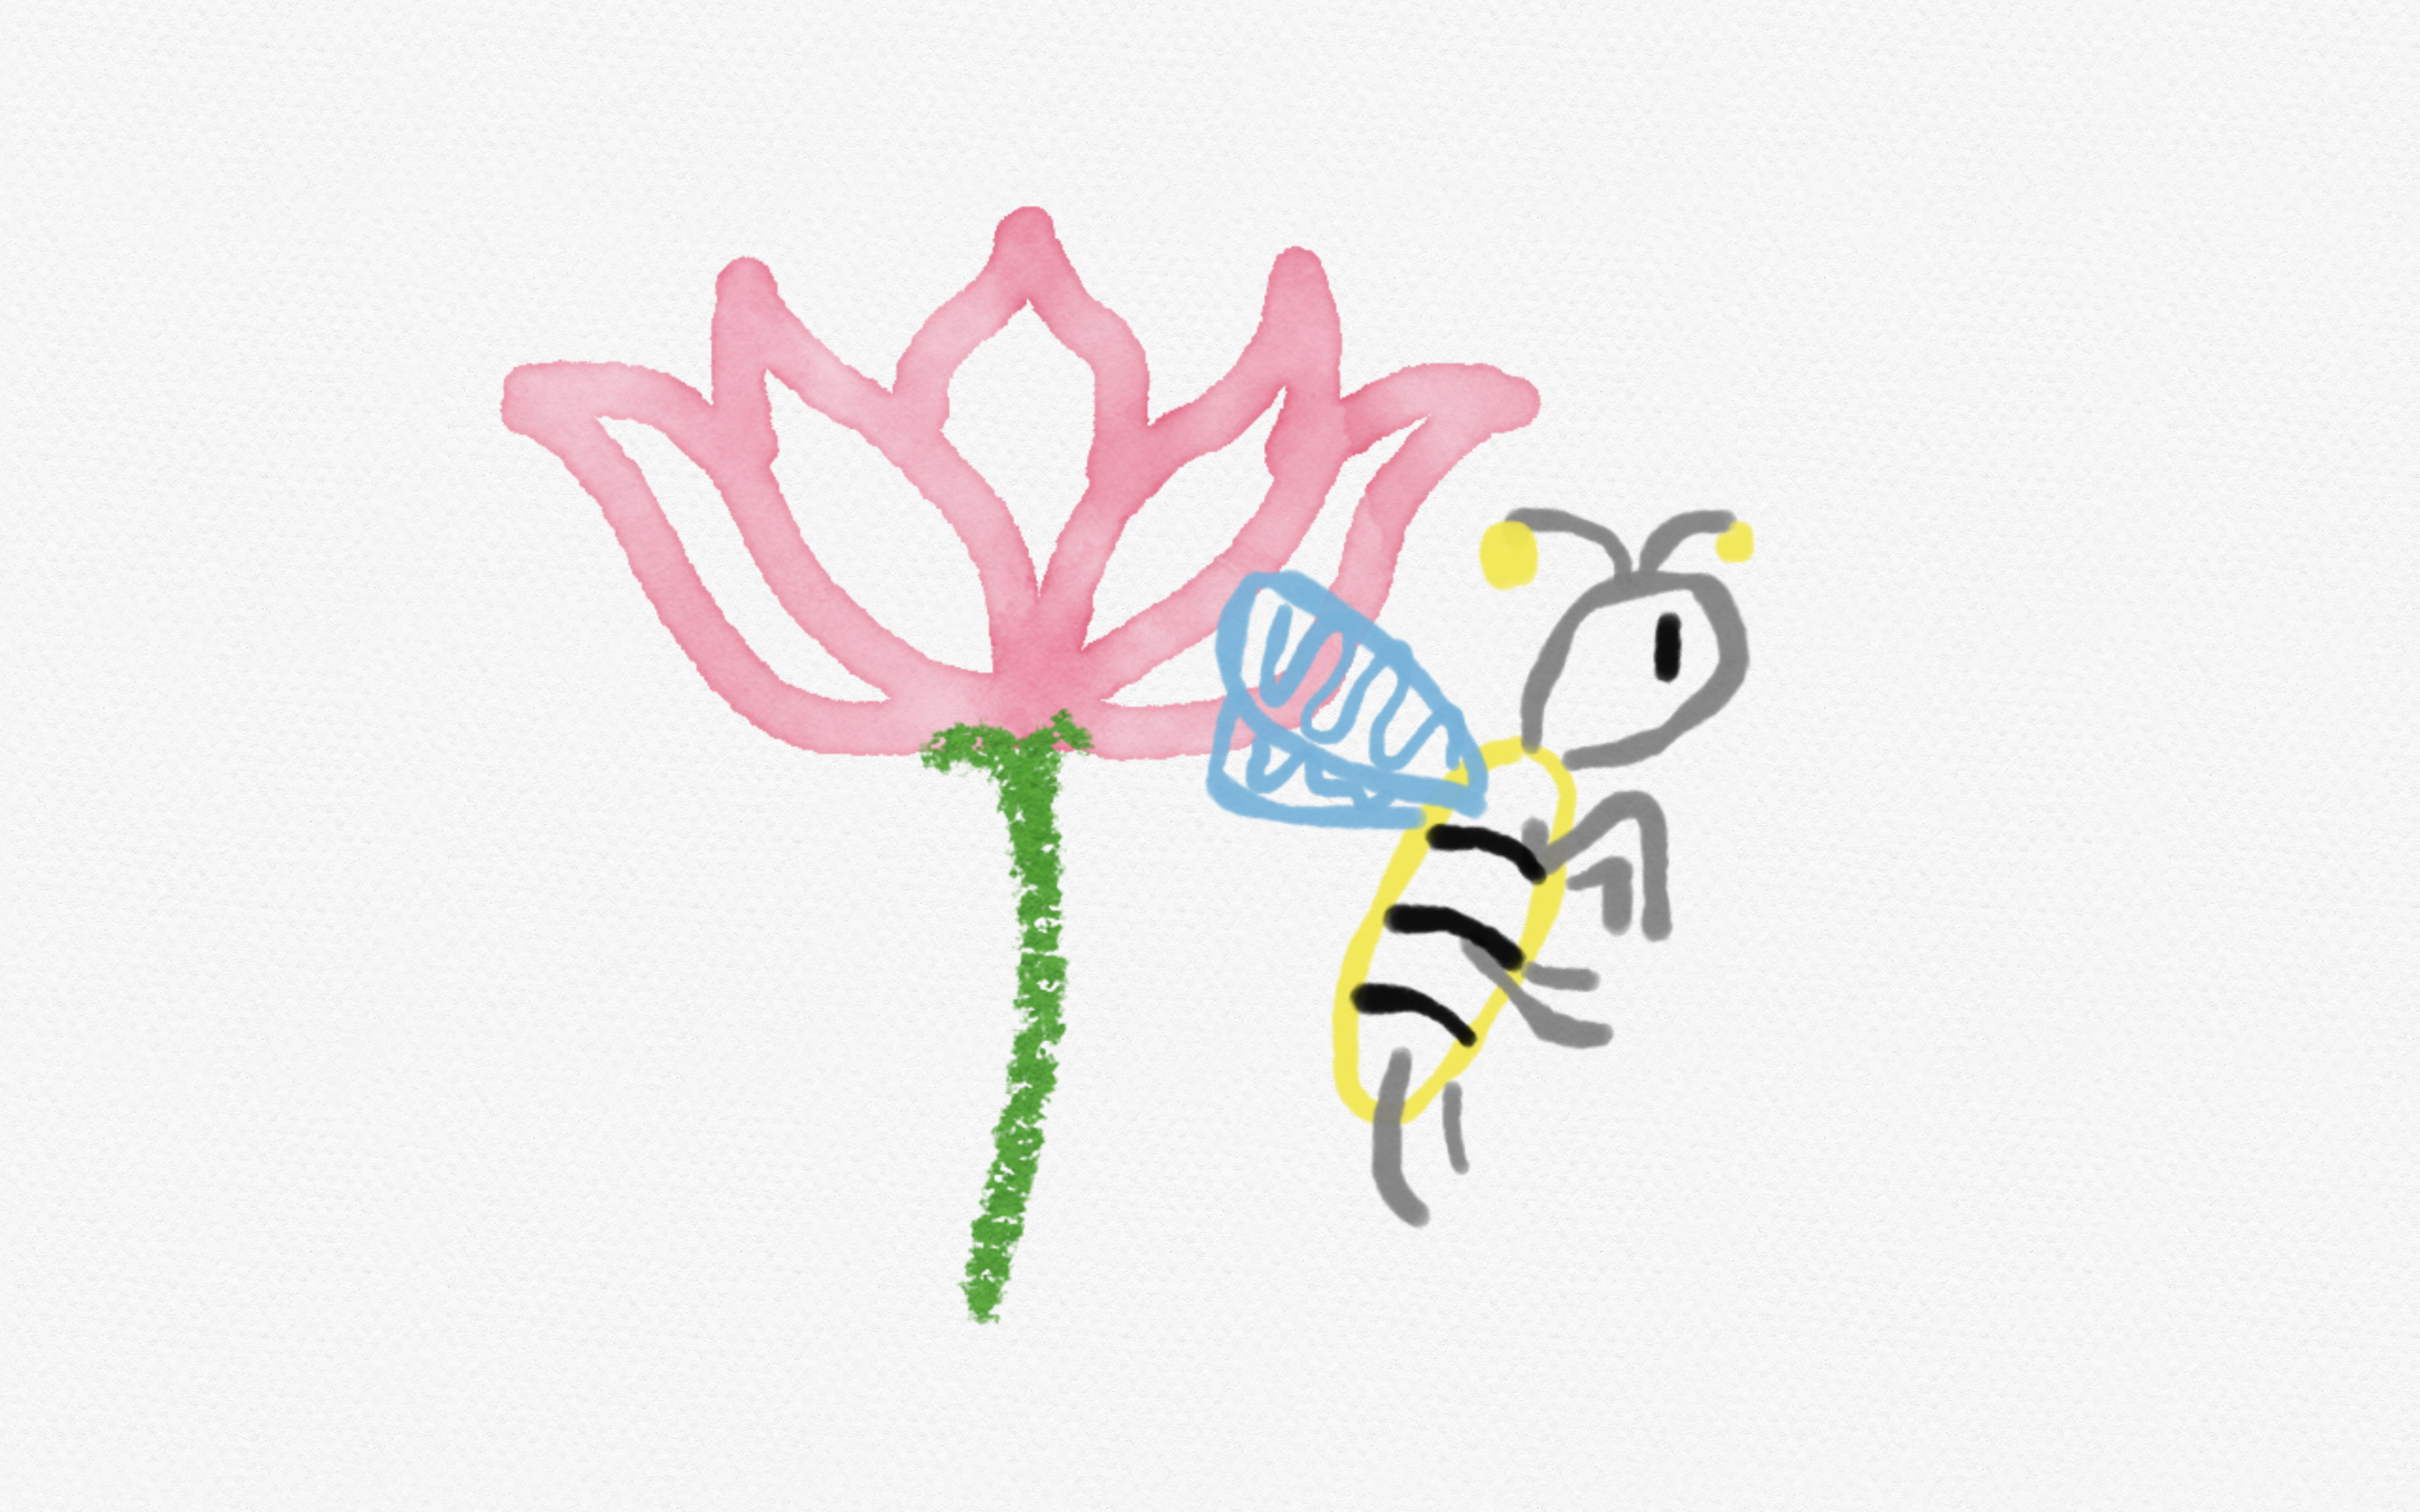
\includegraphics[width = 30em]{Logo}
\end{figure}
\newpage
\tableofcontents
\newpage

%----------------------------------------------------------------------Kapitel 1--------------------------------------------------------------------------------------------

\section{Milestones}

%----------------------------------------------------------------------Kapitel 2--------------------------------------------------------------------------------------------

\section{Arbeitspakete}

%----------------------------------------------------------------------Kapitel 3--------------------------------------------------------------------------------------------

\section{PERT-Diagramm}

%----------------------------------------------------------------------Kapitel 4--------------------------------------------------------------------------------------------

\section{Spezialgebiete}

%----------------------------------------------------------------------Kapitel 5--------------------------------------------------------------------------------------------
\newpage
\section{Whitebox-Tests}
\sectionauthor{Sergei Pravdin}
Ein Entwickler implementiert nicht nur Arbeitspakete, für die er zuständig ist, sondern auch entsprechende für diese Arbeitspakete Whitebox-Test, um etwaige Bugs sofort in Quell-Code zu korrigieren. Whitebox-Test werden klassisch (nach der Implementierung der Klassen) und ohne TDD geschrieben. Die Arbeitspakete werden durch die Verbindung mit der Datenbank getestet, wenn der Zustand der Anwendung es ermöglicht. Sonst werden fehlende Bestandteile von Mockito oder PowerMock gemockt. Jedes Arbeitspaket hat mindestens einen Testfall. Die Tests werden mit dem Projekt mitgeliefert. Die im Folgenden beschriebenen Testfälle bauen aufeinander auf. Das bedeutet, dass der Zustand des Systems für den folgenden Testfall übernommen wird. Vor dem Projektabgabe werden die allen erzeugenden beim Testing Objekte aus der Datenbank manuell gelöscht. 

­\subsection{Milestone 1}

\subsubsection{Meta-implementation - Logger.}
Für den Test des Loggers bekommen wir zuerst getInstance() und rufen die Methode development(''testMessage'') auf. Der Test ist bestanden, wenn das Ergebnis der Methode getMessage() ''testMessage'' ist.

\subsubsection{Meta-implementation - ConfigReader}
Um den ConfigReader zu testen, bekommen wir getInstance() und rufen getSystemConfigurations() auf. Als Ergebnis wird ein eine richtige Config-Propertie erwartet.

\subsubsection{Utilities I}
Der Test ist für ein ApplicationDao zuständig. Ein ApplicationDto 'testDto' wird erstellt und durch testDto.setName(''testName'') ausgefüllt. Danach wird eine Methode \linebreak ApplicationDao.createCustomization(testDto) aufgerufen. Der Test ist bestanden, wenn eine Methode ApplicationDao.readCustomization(testDto).getName() ''testName'' ist.

\subsubsection{Utilities II - TokenGenerator}
Zuerst wird ein TokenDto tokenDto erzeugt. Dann wird tokenDto durch tokenDto = TokenGenerator.generateToken() ausgefüllt. Der Test ist bestanden, falls tokenDto.getContent() nicht null ist.

\subsubsection{System Start}
Die Methode DataLayerInitializer.setUpConnectionPool() wird aufgerufen. Der Test ist bestanden, wenn ConnectionPool.getInstance() nicht null ist.

\subsubsection{Facelets}
Eine Methode logOut() von einem Footer wird aufgerufen. Der Test ist bestanden, wenn das Ergebnis ''logIn.xhtml?faces-redirect=true'' ist.

\subsubsection{Exception handling}
Wir wollen eine Fehlerseite testen, deshalb wird ErrorDto 'testErrorDto' erzeugt und durch setMessage(''testErrorMessage'') ausgefüllt. Dann wird eine Methode setErrorDto(testErrorDto) aufgerufen. Der Test ist bestanden, wenn das Ergebnis der Methode getMessage() von der Klasse 'Error' ''testErrorMessage'' ist.

\subsubsection{User definition - Registrierung}
Ein UserDto 'userDto' wird erzeugt. Dann werden eine Methode userDto.setId(1), \linebreak userDto.setPassword(testPassword) und userDto.setEmailAddress(testSep21email@gmail.com) aufgerufen. Im nächsten Schritt wird die Methode 'register()' in der Klasse 'Registration' aufgerufen. Diese Methode muss eine Interaktion mit einem UserDao, genauer gesagt mit der Methode 'UserDao.createUser(userDto)', implementieren, deshalb ist der Test bestanden, wenn das Ergebnis der Methode 'UserDao.readUserByEmail(userDto).getId()'  ''1'' ist (Das bedeutet, das ein neuer Nutzer mit der Id ''1'' in der Datenbank erfolgreich abgespeichert ist).

\subsubsection{User Authentication - LogIn (erfolglos)}
Eine Methode setEmail(wrongEmail) und eine Methode setPassword(wrongPassword) aus der Klasse Login werden aufgerufen. Im nächsten Schritt wird eine Methode logIn() aufgerufen. Das Ergebnis muss ''null'' sein, damit der Test als bestanden gilt. 

\subsubsection{User Authentication - LogIn (erfolgreich)}
Eine Methode setEmail(testSep21email@gmail.com) und eine Methode setPassword(testPassword) aus der Klasse Login werden aufgerufen. Im nächsten Schritt wird eine Methode logIn() aufgerufen. Das Ergebnis muss ''profile?id=1'' sein, damit der Test als bestanden gilt.

\subsubsection{User Authentication - User Delete}
Ein UserDto 'userDto' wird erzeugt. Dann werden eine Methode userDto.setId(1), \linebreak userDto.setPassword(testPassword) und userDto.setEmailAddress(testSep21email@gmail.com) aufgerufen. Im nächten Schritt wird eine Methode readUserByEmail(userDto).
Ein erhaltenes UserDto wird wieder durch die Methode UserDao.deleteUser(userDto) übergeben. Der Test ist bestanden, wenn das Ergebnis der Methode UserDao.readUserByEmail(userDto) ''null'' ist. Das bedeutet, dass kein Nutzer mit der ID '1' in der Datenbank existiert. Am Schluss wird einen Test 'User definition - Registration' wieder aufgerufen, um einen Nutzer für weitere Test zur Verfügung zu stellen.

\subsubsection{App management, global - Change contact information}
Ein ApplicationDto 'testDto' wird erzeugt. Dann wird die Methode setApplication(testDto) aus der Klasse 'Contact' aufgerufen. Im nächsten Schritt werden die Methode testDto.setCity(''testCity'') und save() aus der Klasse 'Contact' aufgerufen. Der Test gilt als bestanden, wenn die Methode getApplication().getCity() aus der Klasse 'Contact' das Ergebnis ''testCity'' liefert.


\subsubsection{Administrative functions}
Ein ApplicationDto 'testDto' wird erzeugt. Dann wird die Methode setApplication(testDto) aus der Klasse 'Administration' aufgerufen. Im nächsten Schritt werden die Methode \linebreak testDto.setSiteNotice(''testNotice'') und save() aus der Klasse 'Administration' aufgerufen. Der Test gilt als bestanden, wenn die Methode getApplication().getSiteNotice() aus der Klasse 'Administration' das Ergebnis ''testNotice'' liefert.

­\subsection{Milestone 2}
\subsubsection{User profile - Änderung einer Hausnummer}
Ein UserDto 'userDto' wird zuerst erzeugt, dann wird die Methode \linebreak userDto.setEmailAddress(''testSep21email@gmail.com'') aufgerufen und andere Attribute von userDto werden durch userDto = UserDao.readUserByEmail(userDto) ausgefüllt. Im nächsten Schritt wird die Methode setUser(userDto) aus der Klasse 'Profile' aufgerufen. Dann wird sich eine Hausnummer durch userDto.setStreetNumber(''13a'') geändert. Abschießend wird die Methode 'save()' aufgerufen. Jetzt muss die neue Hausnummer in der Datenbank durch das userDto von der Klasse 'Profile' aktualisiert. Der Test ist bestanden, wenn die Methode \linebreak UserDao.readUserByEmail(userDto).getStreetNumber() das Ergebnis ''13a'' liefert.

\subsubsection{Medium attributes - Löschen eines Attributes}
Ein Map<Integer, AttributeDto> 'attributes' wird gemockt. Ein neues AttributeDto 'testDto' wird erzeugt und eine Methode testDto.setId(1) aufgerufen. Danach wird ein 'testDto' durch attributes.put(1, testDto) hinzugefügt. Im nächsten Schritt wird eine Methode setAttributes(attributes) aus der Klasse 'MediumSchemaEditor' aufgerufen. Schließlich wird eine testende Methode deleteAttribute(1) aufgerufen. Der Test ist bestanden, wenn die Methode aus der Klasse 'MediumSchemaEditor' getAttributes.get(1) 'null' liefert.

\subsubsection{Medium management - Erstellung eines Mediums}
Ein UserDto 'userDto' wird zuerst erzeugt, dann wird die Methode \linebreak setEmailAddress(''testSep21email@gmail.com'') aufgerufen und andere Attribute von userDto werden durch userDto = UserDao.readUserByEmail(userDto) ausgefüllt. Im nächsten Schritt wird die Methode setUser(userDto) aus der Klasse 'MediumCreator' aufgerufen. Danach werden ein mediumDto mit der ID '1', dem Name 'testMedium' und ein CopyDto mit der ID '2' erstellt. Im nächsten Schritt werden die Methoden setMedium und setCopy in der Klasse 'MediumCreator' aufgerufen. Schließlich wird die Methode createMediumAndFirstCopy() aufgerufen. Der Test ist bestanden, wenn die Methode MediumDao.readMedium(mediumDto).getId() das Ergebnis '1' liefert.

\subsubsection{Medium management - Ausleihe eines Exemplars durch einen Nutzer}
Ein UserDto 'userDto' wird zuerst erzeugt, dann wird die Methode \linebreak setEmailAddress(''testSep21email@gmail.com'') aufgerufen und andere Attribute von userDto werden durch userDto = UserDao.readUserByEmail(userDto) ausgefüllt. Im nächsten Schritt wird die Methode setUser(userDto) aus der Klasse 'Medium' aufgerufen. Danach werden ein mediumDto mit der ID '1', eine Liste 'copies' und ein CopyDto mit der ID '2' erstellt. Im nächsten Schritt werden die Methoden setMedium und copies.put(1, copyDto) in der Klasse 'MediumCreator' aufgerufen. Schließlich wird die testende Methode pickUpCopy(1, userDto) aufgerufen. Der Test ist bestanden, wenn die Methode MediumDao.readMedium(mediumDto).getCopy(1).getCopyStatus() das Ergebnis 'READY FOR PICKUP' liefert.

\subsubsection{Category search - Erstellung einer Kategorie}
Zuerst wird ein categoryDto erzeugt und durch categoryDto.setId(3) und \linebreak categoryDto.setName(''testCategory'') ausgefüllt. Dann wird eine Methode \linebreak setCategory(categoryDto) in der Klasse 'CategoryCreator' aufgerufen. Schließlich wird eine testende Methode createCategory() aufgerufen. Der Test ist bestanden, wenn die Methode \linebreak CategoryDao.readCategory(categoryDto).getName() das Ergebnis ''testCategory'' liefert.

\subsubsection{Medium transactions - Direktausleihe eines Exemplars durch einen Mitarbeiter}
Ein UserDto 'userDto' wird zuerst erzeugt, dann wird die Methode \linebreak setEmailAddress(''testSep21email@gmail.com'') aufgerufen und andere Attribute von userDto werden durch userDto = UserDao.readUserByEmail(userDto) ausgefüllt. Im nächsten Schritt wird die Methode setUser(userDto) aus der Klasse 'DirectLending' aufgerufen. Dann werden ein copyDto und ein mediumDto erzeugt. Sie werden durch copyDto.setId(2) und mediumDto.setId(1) definiert. Dann wird ein copyDto durch eine Methode MediumDao.readMedium(mediumDto).getCopies(1) ausgefüllt und durch eine Methode copies.put(copyDto) in der Klasse 'DirectLending' hinzugefügt. Schließlich wird eine testende Methode lendCopy(2, userDto) aufgerufen. Der Test ist bestanden, wenn die Methode MediumDao.readMedium(mediumDto).getCopy(1).getCopyStatus() das Ergebnis 'BORROWED' liefert.

\subsubsection{MaintenanceProcess}
Der Test ist bestanden, wenn MaintenanceProcess.getInstance() nicht 'null' ist.

­\subsection{Milestone 3}
\subsubsection{Medium search}
Ein MediumSearchDto 'mediumSearch' wird erzeugt und durch \linebreak mediumSearch.setGeneralSearchTerm(''testMedium'') ausgefüllt. Im nächsten Schritt wird eine Methode setMediumSearch(mediumSearch) in der Klasse 'MediumSearch' aufgerufen. Schließlich wird eine testende Methode searchMedium() aufgerufen. Der Test ist bestanden, wenn eine Methode getItems() in der Klasse 'MediumSearch' ein mediumDto mit einem Attribut 'testMedium' liefert.

\subsubsection{Password and email revalidation - Zurücksetzung eines Passwords}
Ein UserDto 'userDto' wird zuerst erzeugt, dann wird die Methode \linebreak setEmailAddress(''testSep21email@gmail.com'') aufgerufen und andere Attribute von userDto werden durch userDto = UserDao.readUserByEmail(userDto) ausgefüllt. Im nächsten Schritt wird die Methode setUser(userDto) aus der Klasse 'PasswordReset' aufgerufen.
Die Attribute einer Klasse 'PasswordReset' werden durch setPassword(''newPassword'') und \linebreak setConfirmedPassword(''newPassword'') ausgefüllt. Ein TokenDto wird von einem TokenGenerator erstellt und durch setToket(tokenDto) hinzugewiesen. Dann wird eine testende Methode resetPassword(userDto) aufgerufen. Um zu testen, werden eine Methode setEmail(testSep21email@gmail.com) und eine Methode setPassword(newPassword) aus der Klasse 'Login' aufgerufen. Im nächsten Schritt wird eine Methode logIn() aufgerufen. Das Ergebnis muss ''profile?id=1'' sein, damit der Test als bestanden gilt (Erfolgreiche Anmeldung mit einem neuen Password).

\subsubsection{Media by user, individual - Ausgeliehene Exemplare}
Ein UserDto 'userDto' wird zuerst erzeugt, dann wird die Methode \linebreak setEmailAddress(''testSep21email@gmail.com'') aufgerufen und andere Attribute von userDto werden durch userDto = UserDao.readUserByEmail(userDto) ausgefüllt. Im nächsten Schritt wird die Methode setUser(userDto) aus der Klasse 'BorrowedCopies' aufgerufen. Eine testende Methode 'loadCopies()' wird aufgerufen. Der Test ist bestanden, wenn ein Ergebnisliste einer Methode getItems() ein Copy mit der Id '2' beinhaltet.

\subsubsection{Media by user, global - Leifristverstöße}
Zuerst wird ein MediumDto 'mediumDto' erstellt und durch mediumDto.setId(1) identifiziert. Dann wird ein mediumDto durch mediumDto = MediumDao.readMedium(mediumDto) ausgefüllt. Jetzt wird ein CopyDto copyDto erzeugt und durch copyDto = mediumDto.getCopy(2) ausgefüllt (Ein entsprechendes Medium und sein Exemplar wurden in oben definierten Tests in der Datenbank gespeichert). Jetzt wollen wir einen neuen Abgabefrist durch copyDto.setDeadline(''Derzeit + 10 Sekunden'') definieren und diese Änderung in der Datenbank durch MediumDao.update(mediumDto) speichern. Danach wird eine Pause für 11 Sekunden im Test durchgeführt. Jetzt sind wir bereit eine Klasse 'LendingPeriodViolation' zu testen. Der Test ist bestanden, wenn sich ein copyDto mit der Id '2' im Ergebnis der Methode getItems() der Klasse 'LendingPeriodViolation' befindet.

\subsubsection{User search}
Ein userSearchDto wird erstellt und eine Methode \linebreak userSearchDto.setSearchTerm(''testSep21email@gmail.com'') aufgerufen. Danach wird eine Methode setUserSearchDto(userSearchDto) aus der Klasse 'UserSearch' aufgerufen. Im nächsten Schritt wird eine testende Methode searchUser() aufgerufen und eine Methode getItems() aus der Klasse 'UserSearch' muss im Ergebnis ein userDto mit der Id '1' beinhalten, damit der Test bestanden ist. 

\end{document}
